\documentclass[CJKutf8,xcolor=pdftex,dvipsnames,table]{beamer}
\usepackage{hyperref}
\hypersetup{
  pdftitle={Operating System Concepts},
  pdfauthor={Hong MingJian},
  pdfsubject={Virtual Memory},
  pdfpagemode={FullScreen},
  colorlinks={true},
  linkcolor={blue},
}
\usepackage{CJKutf8}
\usepackage{mathptmx} %https://forum.ubuntu.com.cn/viewtopic.php?f=35&t=269943

\usetheme{Madrid}%{Warsaw}
\usecolortheme{crane}

%gets rid of bottom navigation bars
\setbeamertemplate{footline}[page number]{}
%gets rid of navigation symbols
\setbeamertemplate{navigation symbols}{}

\begin{document}
\begin{CJK*}{UTF8}{song}

  \title{操作系统原理}
  \subtitle{第十章:虚拟内存}
  \author{洪明坚}
  \institute{重庆大学软件学院}
  \date{\today}

  \AtBeginSection[]
  {
    \begin{frame}
      \frametitle{Outline}
      \tableofcontents[currentsection]
    \end{frame}
  }

  \frame{\titlepage}
  \frame{\frametitle{目录}\tableofcontents}
  
  \section{Introduction}
  
  %% PAGE
  \begin{frame}
    \frametitle{Background(1/2)} \pause
    \begin{itemize}
    \item{IBM's poster explaining virtual memory in 1978: } \pause
      \begin{itemize}
      \item{If it's there and you can see it, it's real;} \pause
      \item{If it's there and you can't see it, \pause it's transparent;} \pause
      \item{If it's not there and you can see it, \pause it's virtual;} \pause
      \item{If it's not there and you can't see it, \pause you erased it!}
      \end{itemize}
    \end{itemize}
  \end{frame}
  
  %% PAGE
  \begin{frame}
    \frametitle{Background(2/2)} \pause
    \begin{itemize}\parskip=0pt
    \item{自从有了计算机以来,我们就希望能够方便、高效地使用(今天仍然)十分有限的内存:} \pause
      \begin{itemize}\parskip=0pt
      \item{用户总是可以认为自己计算机的内存大到足够运行任何程序;} \pause
      \item{程序员可以认为自己的程序将运行在巨大、连续的内存中;} \pause
        \begin{itemize}\parskip=0pt
        \item{不需要用overlay或swap等技术来自己管理内存。} \pause
        \end{itemize}
      \item{进程在运行过程中不能访问(包括读写)其他进程的数据;} \pause
        \begin{itemize}\parskip=0pt
        \item{更不能访问属于操作系统的数据;} \pause
        \item{而且某一个进程引起的问题不会波及到操作系统或其他进程。} \pause
        \end{itemize}
      \item{由于内存有限,应该尽可能地共享一些公用的代码和数据。} \pause
      \end{itemize}
    \item{前面介绍的各种技术解决了上述问题的某一些方面,但没有提出一个整体的解决方案。} \pause
      \begin{itemize}
      \item{虚拟内存技术基于已有的各种技术给出了一个完整的解决方案,是20世纪计算机技术最重要的发明之一。}
      \end{itemize}
    \end{itemize}
  \end{frame}
  
  %% PAGE
  \begin{frame}
    \frametitle{What's virtual memory?(1/2)} \pause
    \begin{itemize}
    \item{\textbf{Virtual memory} is the separation of user logical memory from physical memory.} \pause
      \begin{itemize}
      \item{Provides a huge, continuous and private logical memory, which may be much larger than the physical memory, to \textbf{each} process. } \pause
        \begin{itemize}
        \item{Only part of the program needs to be in memory for execution.} \pause
        \end{itemize}
      \item{Allows address spaces to be shared by several processes.} \pause
        \begin{itemize}
        \item{More efficient process creation.} \pause
        \end{itemize}
      \end{itemize}
    \item{Virtual memory can be implemented via:} \pause
      \begin{itemize}
        % \pausecolors{cyan}{red}{black}
      \item{\textcolor{red}{Demand paging}} \pause
      \item{Demand segmentation}
      \end{itemize}
    \end{itemize}
  \end{frame}
  
  %% PAGE
  \begin{frame}
    \frametitle{What's virtual memory(2/2)} \pause
    \begin{center}
      \includegraphics[scale=.3]{v6f10-1}
    \end{center}
  \end{frame}
  
  \section{Demand paging}
  
  %% PAGE
  \begin{frame}
    \frametitle{Demand paging} \pause
    \begin{itemize}
    \item{Bring a page into memory only when it is needed, i.e., \textbf{lazy swapper}.} \pause
      \begin{itemize}
      \item{Less I/O needed;} \pause
      \item{Less memory needed;} \pause
      \item{Faster response;} \pause
      \item{More processes;} \pause
      \end{itemize}
    \item{一般情况下,我们用swapper表示整个进程的交换;而用pager来表示对页进行交换的lazy swapper。}
    \end{itemize}
  \end{frame}
  
  %% PAGE
  \begin{frame}
    \frametitle{Pager} \pause
    \begin{center}
      \includegraphics[scale=.3]{v6f10-2}
    \end{center}
  \end{frame}
  
  %% PAGE
  \begin{frame}
    \frametitle{When to bring in a page?} \pause
    \begin{itemize}
    \item{当操作系统调度某个进程运行时,如何判断该进程的页面是否已经被映射到内存中?} \pause
    \item{Remember: With each page table entry (PTE) a valid-invalid bit is associated: } \pause
      \begin{itemize}
      \item{If the bit is set to ``valid'', it indicates that the associated page is both legal and in memory;} \pause
      \item{Otherwise, it indicates the page is not legal (i.e., not in the
          logical address space of the process), or is legal but currently
          not in memory.}
      \end{itemize}
    \end{itemize}
  \end{frame}
  
  %% PAGE
  \begin{frame}
    \frametitle{Valid-Invalid bit} \pause
    \begin{center}
      \includegraphics[scale=.3]{v6f10-3}
    \end{center}
  \end{frame}
  
  %% PAGE
  \begin{frame}
    \frametitle{What happens if not in memory?} \pause
    \begin{itemize}
    \item{During address translation in MMU, if valid-invalid bit in PTE is ``invalid'', } \pause
      \begin{itemize}
      \item{CPU triggers a \textbf{page-fault trap} into the OS,} \pause
      \item{then OS looks at an internal table (usually kept in the PCB) to decide if it's } \pause
        \begin{itemize}
        \item{an illegal reference, OS terminates the process;} \pause
        \item{legal but not in memory, OS will bring it in.}
        \end{itemize}
      \end{itemize}
    \end{itemize}
  \end{frame}

  \subsection{Page-fault}
  
  %% PAGE
  \begin{frame}
    \frametitle{Page-fault service routine(1/2)} \pause
    \begin{enumerate}\parskip=0pt
    \item{We check an internal table for this process to determine whether the
        reference was a legal or illegal memory access;} \pause
    \item{If the reference was illegal, we terminate the process. If it was
        legal, but we have not yet brought in that page, we now page it in;} \pause
    \item{We find a free frame;} \pause
    \item{We schedule a disk operation to read the desired page into the newly allocated frame} \pause
    \item{When the disk read is complete, we modify the page table kept with the process to indicate that the page is now in memory;} \pause
    \item{We restart the instruction that was interrupted by the page-fault trap. The process can now access the page \textbf{as if} it had always been in memory.}
    \end{enumerate}
  \end{frame}
  
  %% PAGE
  \begin{frame}
    \frametitle{Page-fault service routine(2/2)} \pause
    \begin{center}
      \includegraphics[scale=.3]{v6f10-4}
    \end{center}
  \end{frame}
  
  %% PAGE
  \begin{frame}
    \frametitle{Architecture requirements} \pause
    \begin{enumerate}
    \item{Page Table: This table has the ability to mark an entry invalid through a valid-invalid bit;} \pause
    \item{Secondary memory: This memory holds those pages that are not present in main memory. It's usually called \textbf{swap space};} \pause
    \item{Capability to restart any instruction \textbf{exactly} after a page-fault.} \pause
      \begin{itemize}
      \item{This is \textbf{NOT} easy sometime.}
      \end{itemize}
    \end{enumerate}
  \end{frame}
  
  %% PAGE
  \begin{frame}
    \frametitle{Questions}
    \begin{itemize}
    \item{Any questions?}
    \end{itemize}
    \begin{center}
      \includegraphics[scale=.5]{question}
    \end{center}
  \end{frame}

  \subsection{Page replacement}
  
  %% PAGE
  \begin{frame}
    \frametitle{What happens if no free frame?} \pause
    \begin{itemize}
    \item{While the process executes and accesses pages that are in memory, execution proceeds normally.} \pause
    \item{By increasing the degree of multiprogramming, we will \textbf{over-allocate} the physical memory. When page fault occurs, no free frames available. How to proceed?} \pause
    \item{Find a frame in memory, but not actively in use, page it out.} \pause
      % \item{We need a \textbf{page replacement algorithm}} \pause
      %   \begin{itemize}
      %   \item{to determine which frame should be swapped out (replaced),} \pause
      %   \item{which will result in minimum number of page faults. } \pause
      %   \end{itemize}
    \item{Here comes the \textbf{Page replacement}} \pause
      \begin{itemize}
      \item{Prevent over-allocation of memory by modifying page-fault service routine to include page replacement.} \pause
      \item{\textbf{Page replacement completes that large virtual memory can be provided on a smaller physical memory.}}
      \end{itemize}
    \end{itemize}
  \end{frame}
  
  %% PAGE
  \begin{frame}
    \frametitle{Page replacement} \pause
    \begin{center}
      \includegraphics[scale=.3]{v6f10-6}
    \end{center}
  \end{frame}
  
  %% PAGE
  \begin{frame}
    \frametitle{Page-fault service routine including page replacement(1/2)} \pause
    \begin{itemize}
    \item{We should modify the page-fault service routine to include page replacement.} \pause
      \begin{enumerate}
      \item{Find the location of the desired page on the disk;} \pause
      \item{Find a free frame: } \pause
        \begin{enumerate}
        \item{If there is a free frame, use it; else} \pause
        \item{Use a \textbf{page-replacement algorithm} to select a \textbf{victim} frame;} \pause
        \item{Write the victim page to the disk; change the PTE accordingly.} \pause
        \end{enumerate}
      \item{Read the desired page into the (newly) free frame; change the PTE;} \pause
      \item{Restart the instruction.}
      \end{enumerate}
    \end{itemize}
  \end{frame}
  
  %% PAGE
  \begin{frame}
    \frametitle{Page-fault service routine including page replacement(2/2)} \pause
    \begin{center}
      \includegraphics[scale=.3]{v6f10-7}
    \end{center}
  \end{frame}
  
  %% PAGE
  \begin{frame}
    \frametitle{Refinement} \pause
    \begin{itemize}
    \item{Notice that, if no frames are free, two page transfers are required: } \pause
      \begin{itemize}
      \item{One write and one read} \pause
      \end{itemize}
    \item{We can reduce this overhead by associating each page a \textbf{modify} bit (or \textbf{dirty} bit)} \pause
      \begin{itemize}
      \item{Whenever a page was modified, the hardware will set this bit.} \pause
      \item{The page-out is only needed if dirty bit is set.}
      \end{itemize}
    \end{itemize}
  \end{frame}
  
  %% PAGE
  \begin{frame}
    \frametitle{Example dirty bit} \pause
    \begin{itemize}
    \item{PTE of IA-32} \pause
    \end{itemize}
    \begin{center}
      \includegraphics[scale=.5]{x86pte}
    \end{center}
  \end{frame}
  
  %% PAGE
  \begin{frame}
    \frametitle{Questions}
    \begin{itemize}
    \item{Any questions?}
    \end{itemize}
    \begin{center}
      \includegraphics[scale=.5]{question}
    \end{center}
  \end{frame}

  %% PAGE
  \begin{frame}
    \frametitle{Page-replacement algorithm} \pause
    \begin{itemize}
    \item{算法目标:} \pause
      \begin{itemize}
      \item{Lowest page-fault rate} \pause
      \end{itemize}
    \item{为了方便研究各种页面置换算法,计算各个算法所产生的page fault,引入如下概念:} \pause
      \begin{itemize}
      \item{\emph{Reference string} \pause - the string of memory references. \pause 通常以页面为单位。} \pause
      \end{itemize}
    \item{Evaluate an algorithm by running it on a reference string and computing the number of page faults on that string.} \pause
      \begin{itemize}
      \item{In all following examples, the reference string is\\7, 0, 1, 2, 0, 3, 0, 4, 2, 3, 0, 3, 2, 1, 2, 0, 1, 7, 0, 1}
      \end{itemize}
    \end{itemize}
  \end{frame}
  
  %% PAGE
  \begin{frame}
    \frametitle{Page faults versus the number of frames} \pause
    \begin{center}
      \includegraphics[scale=0.4]{v6f10-8}
    \end{center}
  \end{frame}
  
  %% PAGE
  \begin{frame}
    \frametitle{Questions}
    \begin{itemize}
    \item{Any questions?}
    \end{itemize}
    \begin{center}
      \includegraphics[scale=.5]{question}
    \end{center}
  \end{frame}
  
  %% PAGE
  \begin{frame}
    \frametitle{Various page replacement algorithms} \pause
    \begin{itemize}
    \item{FIFO page replacement} \pause
    \item{Optimal page replacement} \pause
    \item{LRU page replacement} \pause
    \item{Second-chance page replacement}
    \end{itemize}
  \end{frame}
  
  %% PAGE
  \begin{frame}
    \frametitle{FIFO page replacement} \pause
    \begin{itemize}
    \item{Replace the \emph{oldest} page.} \pause
    \item{Example} \pause
      \begin{itemize}
      \item{Page faults with 3 frames.} \pause
      \end{itemize}
    \end{itemize}
    \begin{center}
      \includegraphics[scale=.4]{v6f10-9}
    \end{center}
  \end{frame}
  
  %% PAGE
  \begin{frame}
    \frametitle{Belady's anomaly} \pause
    \begin{itemize}\parskip=0pt
    \item{一般情况下,page-fault会随着frame的数量增加而减少,但是,如果采用FIFO算法,情况有时并非如此。} \pause
    \item{例如,分别在有3和4个frame的系统上引用\\ 1, 2, 3, 4, 1, 2, 5, 1, 2, 3, 4, 5} \pause
    \end{itemize}
    \begin{center}
      \includegraphics[scale=0.2]{v6f10-10} \pause
    \end{center}
    \begin{itemize}
    \item{因此,算法的设计非常重要。}
    \end{itemize}
  \end{frame}
  
  %% PAGE
  \begin{frame}
    \frametitle{Questions}
    \begin{itemize}
    \item{Any questions?}
    \end{itemize}
    \begin{center}
      \includegraphics[scale=.5]{question}
    \end{center}
  \end{frame}
  
  %% PAGE
  \begin{frame}
    \frametitle{Optimal page replacement} \pause
    \begin{itemize}
    \item{Replace the page that will not be used for longest period time.} \pause
    \item{Example} \pause
    \end{itemize}
    \begin{center}
      \includegraphics[scale=0.4]{v6f10-11} \pause
    \end{center}
    \begin{itemize}
    \item{Unfortunately, the optimal page replacement algorithm is difficult to implement because it requires future knowledge of the reference string.}
    \end{itemize}
  \end{frame}
  
  %% PAGE
  \begin{frame}
    \frametitle{LRU page replacement} \pause
    \begin{itemize}\parskip=0pt
    \item{Replace the \emph{least-recently-used} page.} \pause
      \begin{itemize}
      \item{An approximation of the optimal page replacement.} \pause
      \end{itemize}
    \item{Example} \pause
    \end{itemize}
    \begin{center}
      \includegraphics[scale=0.4]{v6f10-12} \pause
    \end{center}
    \begin{itemize}
    \item{The LRU replacement may require substantial hardware assistance to determine an order for the frames defined by the time of last use.}
    \end{itemize}
  \end{frame}
  
  %% PAGE
  \begin{frame}
    \frametitle{Second-chance page replacement (1/4)} \pause
    \begin{itemize}\parskip=0pt
    \item{Few computer system provide sufficient hardware support for true LRU algorithm.} \pause
    \item{For an approximation, some hardware provide some help in the form of a \emph{reference(R)} or \emph{accessed(A)} bit.} \pause
      \begin{itemize}\parskip=0pt
      \item{Whenever a page is accessed, the hardware will set the \emph{R} bit associated with the page.} \pause
      \end{itemize}
    \item{The algorithm works as following} \pause
      \begin{itemize}\parskip=0pt
      \item{When a page has been selected, we inspect its \emph{R} bit.} \pause
        \begin{itemize}\parskip=0pt
        \item{If $R=0$, replace this page;} \pause
        \item{Otherwise, we give it a second chance and move on to select next page.} \pause
        \end{itemize}
      \item{When a page gets a second chance, its \emph{R} bit is cleared.}
      \end{itemize}
    \end{itemize}
  \end{frame}
  
  %% PAGE
  \begin{frame}
    \frametitle{Second-chance page replacement (2/4)} \pause
    \begin{itemize}
    \item{Example reference (or accessed) bit} \pause
    \end{itemize}
    \begin{center}
      \includegraphics[scale=.5]{x86pte}
    \end{center}
  \end{frame}
  
  %% PAGE
  \begin{frame}
    \frametitle{Second-chance page replacement (3/4)} \pause
    \begin{center}
      \includegraphics[scale=0.3]{v6f10-14}
    \end{center}
  \end{frame}
  
  %% PAGE
  \begin{frame}
    \frametitle{Second-chance page replacement (4/4)} \pause
    \begin{itemize}
    \item{Also known as {\em clock} page replacement} \pause
    \end{itemize}
    \begin{center}
      \includegraphics[scale=0.25]{mosv2f4-17}
    \end{center}
  \end{frame}
  
  %% PAGE
  \begin{frame}
    \frametitle{Questions}
    \begin{itemize}
    \item{Any questions?}
    \end{itemize}
    \begin{center}
      \includegraphics[scale=.5]{question}
    \end{center}
  \end{frame}
 
  \subsection{Thrashing}
  
  %% PAGE
  \begin{frame}
  \frametitle{Thrashing (1/2)} \pause
  \begin{itemize}\parskip=0pt
  \item{\emph{Page-fault rate}: $0\leq p \leq 1.0$} \pause
    \begin{itemize}
    \item{if $p=0$, no page faults;} \pause
    \item{if $p=1$, every reference causes a fault.} \pause
    \end{itemize}
  \item{Effective access time (EAT)\\$=(1-p)\times$(memory  access time)$ + p \times $(page fault time)\\ $\approx p \times $(page fault time)} \pause
  \item{If a system does not have ``enough'' frames, the page-fault rate is very high. This leads to:} \pause
  \begin{itemize}
  \item{Low CPU utilization.} \pause
  \item{The admission scheduler thinks that it needs to increase the degree of multiprogramming.} \pause
  \item{More processes are added to the system.} \pause
  \end{itemize}
  \item{\emph{Thrashing} is a situation where a system is busy bringing pages in and out and does nothing useful.}
  \end{itemize}
  \end{frame}

  %% PAGE
  \begin{frame}
  \frametitle{Thrashing (2/2)} \pause
  \begin{center}
  \includegraphics[scale=0.3]{v6f10-15}
  \end{center}
  \end{frame}
  
  %% PAGE
  \begin{frame}
    \frametitle{Why thrashing?} \pause
    \begin{itemize}
    \item{The principle behind the scene} \pause
      \begin{itemize}
      \item{\emph{Locality model}} \pause
        \begin{itemize}
        \item{\emph{Locality} is defined as a set of pages that are actively used in the system.} \pause
        \item{\emph{Process migrates from one locality to another}.} \pause
            \begin{center}
            \includegraphics[scale=.2]{v6f10-16} \pause
            \end{center}
          % \begin{itemize}
          % \item{Localities may overlap.} \pause
          % \end{itemize}
        \end{itemize}
        \item{Locality model is also the reason why the caches work well.} \pause
      \end{itemize}
    \item{Why does thrashing occurs?} \pause
      \begin{itemize}
      \item{$\sum{size\ of\ locality} > total\ memory\ size$}
      \end{itemize}
    \end{itemize}
  \end{frame}
  
  %% PAGE
  \begin{frame}
    \frametitle{Questions}
    \begin{itemize}
    \item{Any questions?}
    \end{itemize}
    \begin{center}
      \includegraphics[scale=.5]{question}
    \end{center}
  \end{frame}
  
  %% PAGE
  \begin{frame}
    \frametitle{Working-set model (1/2)} \pause
    \begin{itemize}
    \item{The \emph{working-set model} is an approximation of the locality model.} \pause
      \begin{itemize}
      \item{It defines a parameter named \emph{working-set window}, $\Delta$, to be the number of page references.} \pause
      \item{The set of pages in the most recent $\Delta$ page references is the \emph{working-set}.} \pause
        \begin{itemize}
        \item{Thus, the working-set is an approximation of the process's locality.} \pause
          % \begin{itemize}
          % \item{If the $\Delta$ is too small, it will not encompass the entire locality;} \pause
          % \item{If the $\Delta$ is too large, it may overlap several localities.} \pause
          % \end{itemize}
        \end{itemize}
      \item{We denote the $WSS_i$ as the working set of process $P_i$ in the most recent $\Delta$.} \pause
        \begin{itemize}
        \item{Then, $D=\sum{WSS_i}$ is the total demand frames.} \pause
        \item{If $D >$ total memory size, the system may be thrashing.}
        \end{itemize}
      \end{itemize}
    \end{itemize}
  \end{frame}
  
  %% PAGE
  \begin{frame}
    \frametitle{Working-set model (2/2)} \pause
    \begin{center}
      \includegraphics[scale=0.4]{v6f10-17}
    \end{center}
  \end{frame}
  
  %% PAGE
  \begin{frame}
    \frametitle{Use of working-set model} \pause
    \begin{itemize}
    \item{The operating system monitors the working-set of each process and allocates to that working-set enough frames to provide it with its working-set size.} \pause
    \item{If there are enough extra frames, new processes can be created; else if the sum of working-set size exceeds the total number of available frames, the OS selects a process to suspend.} \pause
    \item{\emph{The working-set strategy prevents thrashing while keeping the degree of multiprogramming as high as possible.}}
    \end{itemize}
  \end{frame}
  
  %% PAGE
  \begin{frame}
    \frametitle{Questions}
    \begin{itemize}
    \item{Any questions?}
    \end{itemize}
    \begin{center}
      \includegraphics[scale=.5]{question}
    \end{center}
  \end{frame}
  
  \section{Case study}

  \subsection{Address space layout}

  %% PAGE
  \begin{frame}
    \frametitle{Address space layout (1/2)} \pause
    \begin{itemize}
    \item{With the introduction of the virtual memory, a huge, continuous and private address space is reserved to each process in the system.} \pause
      \begin{itemize}
      \item{On a 32-bit architecture, the address space has $2^{32}$ bytes.} \pause
      \item{Because all the processes must access the operating system kernel to request services, the operating system kernel must reside in the address space to be accessible from processes.} \pause
        \begin{minipage}[c]{0.5\textwidth}
          \begin{itemize}
          \item{The part of the space allocated to operating system kernel is called \emph{kernel space}, which is invisible to the process;} \pause
          \item{The rest of the space is called \emph{user space}, which can be used by the process.} \pause
          \end{itemize}
        \end{minipage}%
        \begin{minipage}[c]{0.5\textwidth}
          \begin{center}
            \includegraphics[scale=.4]{asl}
          \end{center}
        \end{minipage}
      \end{itemize}
    \end{itemize}
  \end{frame}

  
  %% PAGE
  \begin{frame}
    \frametitle{Address space layout (2/2)} \pause
    \begin{itemize}
    \item{The layout within the kernel and user space varies from one operating system to another.} \pause
      \begin{itemize}
      \item{For example, which part of user space holds the \emph{text section}, \emph{data section}, \emph{stack} or \emph{heap} of a process.} \pause
      \end{itemize}
    \item{We will take Windows 2000 and Linux as the examples to explain their address space layout.}
    \end{itemize}
  \end{frame}
  
  %% PAGE
  \begin{frame}
    \frametitle{Windows 2000} \pause
    \begin{itemize}
    \item{References:} \pause
      \begin{itemize}
          \item{Mark E. Russinovich and David A. Solomon, Windows Internals ( 
\htmladdnormallink{Part 1}{https://www.microsoftpressstore.com/store/windows-internals-part-1-9780735648739},
\htmladdnormallink{Part 2}{https://www.microsoftpressstore.com/store/windows-internals-part-2-9780735665873}), 6th Edition, Microsoft Press, 2012.} \pause
        \begin{itemize}
        \item{中文版:深入解析Windows操作系统(第6版),潘爱民、范德成 译} \pause
        \end{itemize}
%      \item{Jeffrey Richter, \htmladdnormallink{\emph{Programming Applications for Microsoft Windows}}{http://www.microsoft.com/mspress/books/2345.aspx}, 4th Edition, Microsoft Press, 1999.} \pause
%        \begin{itemize}
%        \item{中文版:Windows核心编程(第4版),王建华 译}
%        \end{itemize}
      \end{itemize}
    \end{itemize}
  \end{frame}
  
  %% PAGE
  \begin{frame}
    \frametitle{Address space layout of Windows 2000 Professional} \pause
    \begin{center}
      \includegraphics[scale=0.4]{2kplayout}
    \end{center}
  \end{frame}
  
  %% PAGE
  \begin{frame}
    \frametitle{Kernel space layout of Windows 2000 Professional} \pause
    \begin{center}
      \includegraphics[scale=0.3]{2kpklayout}
    \end{center}
  \end{frame}

  %% PAGE
  \begin{frame}[fragile]
    \frametitle{User space layout of Windows 20000 Professional} \pause
    \begin{itemize}\parskip=0pt
    \item{Program \htmladdnormallink{VMMap}{https://docs.microsoft.com/en-us/sysinternals/downloads/vmmap} can be used to dump the user space layout of a Windows process} \pause
    \end{itemize}
    \begin{center}
		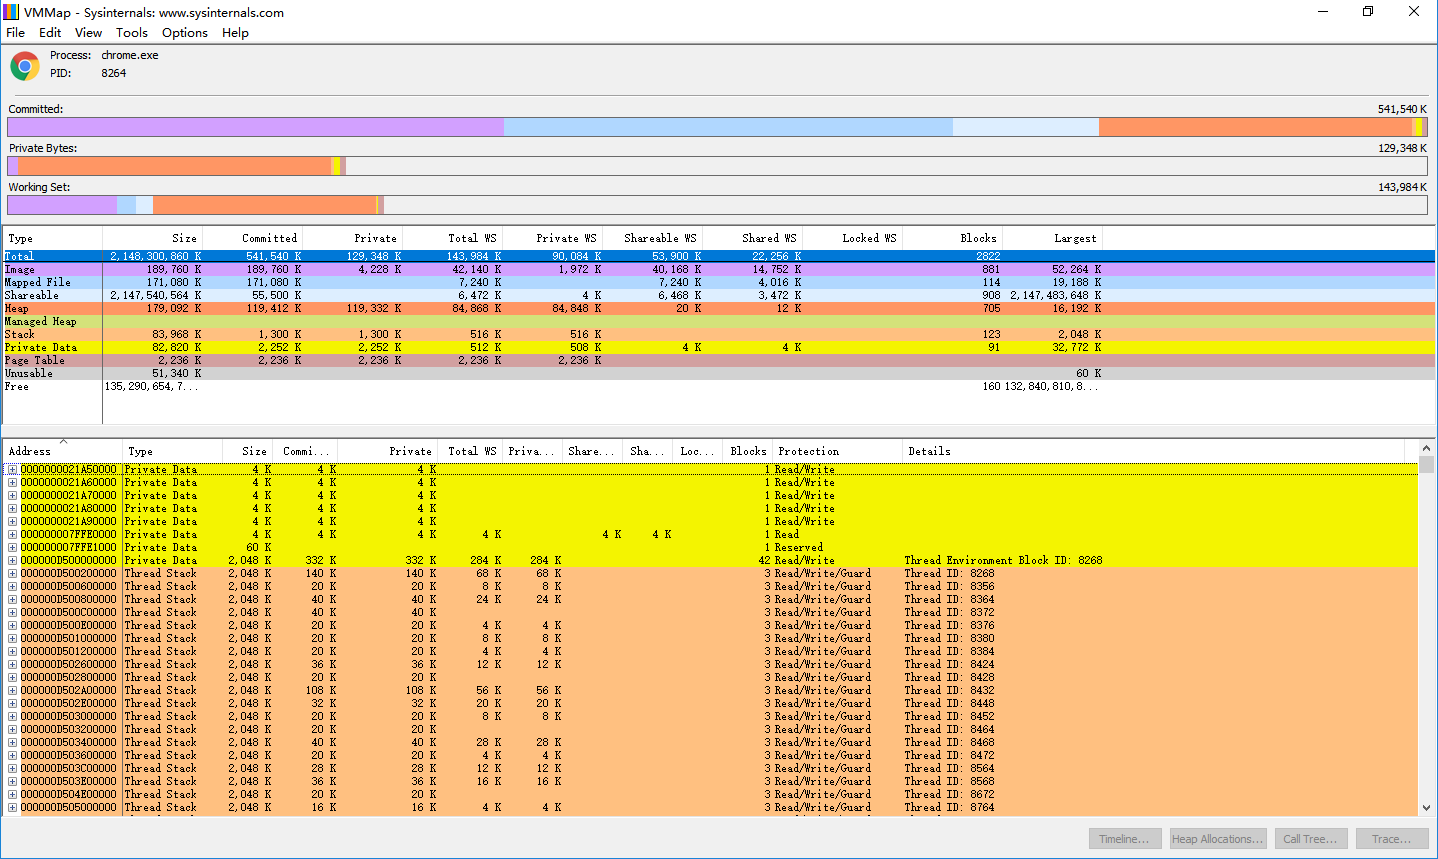
\includegraphics[scale=0.3]{vmmap}
	\end{center}

\iffalse

    {\tiny
\begin{verbatim}
    00010000 Private       4096  1  -RW-
    00020000 Private       4096  1  -RW-
    00030000 Private    1048576  3  -RW- Thread Stack
    00130000 Mapped       12288  1  -R--
    00260000 Mapped       90112  1  -R-- \Device\HarddiskVolume1\WINDOWS\system32\unicode.nls
    00280000 Mapped      249856  1  -R-- \Device\HarddiskVolume1\WINDOWS\system32\locale.nls
    002C0000 Mapped      266240  1  -R-- \Device\HarddiskVolume1\WINDOWS\system32\sortkey.nls
    00310000 Mapped       24576  1  -R-- \Device\HarddiskVolume1\WINDOWS\system32\sorttbls.nls
    00320000 Mapped      266240  1  -R--
    00370000 Private      65536  2  -RW-
    00380000 Mapped       12288  1  -R-- \Device\HarddiskVolume1\WINDOWS\system32\ctype.nls
    00390000 Private      65536  2  -RW-
    00400000 Image        45056  4  ERWC C:\foo.exe
    0040B000 Free     264196096
    10000000 Image        49152  5  ERWC C:\foo.dll
    1000C000 Free    1820278784
    7C800000 Image      1163264  5  ERWC C:\WINDOWS\system32\kernel32.dll
    7C920000 Image       606208  5  ERWC C:\WINDOWS\system32\ntdll.dll
\end{verbatim}
    }

\fi

\end{frame}
  
\iffalse

  %% PAGE
  \begin{frame}
    \frametitle{Address space layout of Windows 2000 Server} \pause
    \begin{minipage}[c]{0.6\textwidth}
      \begin{itemize}
      \item{In the Windows 2000 Advanced Server or DataCenter Server, users can enable 3G user space by adding the ``/3GB'' flag in ``C:$\backslash$boot.ini''.} \pause
      \end{itemize}
    \end{minipage}%
    \begin{minipage}[c]{0.4\textwidth}
      \centering
      \includegraphics[scale=0.3]{2kslayout}
    \end{minipage}
  \end{frame}

\fi
  
  %% PAGE
  \begin{frame}
    \frametitle{Questions}
    \begin{itemize}
    \item{Any questions?}
    \end{itemize}
    \begin{center}
      \includegraphics[scale=.5]{question}
    \end{center}
  \end{frame}
  
  %% PAGE
  \begin{frame}
    \frametitle{Linux} \pause
    \begin{itemize}
    \item{References} \pause
      \begin{itemize}
      \item{Randal E. Bryant, David O' Hallaron, \htmladdnormallink{\emph{Computer System: A Programmer's Perspective}}{http://csapp.cs.cmu.edu/}, John \& Wiley, 2004.} \pause
        \begin{itemize}
        \item{中文版:深入理解计算机系统,龚奕利和雷迎春 译} \pause
        \end{itemize}
      \item{The Linux kernel source code: \url{http://www.kernel.org}.}
      \end{itemize}
    \end{itemize}
  \end{frame}

  %% PAGE
  \begin{frame}
    \frametitle{Address space layout of Linux} \pause
    \begin{center}
      \includegraphics[scale=0.4]{detaillinuxasl}
    \end{center}
  \end{frame}  
  
  %% PAGE
  \begin{frame}[fragile]
    \frametitle{Example} \pause
    \begin{itemize}
    \item{\emph{[hmj@hmj ~]\$ }\textbf{cat /proc/\$(pidof foo)/maps}} \pause
    \end{itemize}
    {\tiny
\begin{verbatim}
        08048000-08049000 r-xp 00000000 00:0d 14446  /home/hmj/foo
        08049000-0804a000 rwxp 00000000 00:0d 14446  /home/hmj/foo
        0804a000-0806b000 rwxp 0804a000 00:00 0      [heap]
        b7e06000-b7e07000 rwxp b7e06000 00:00 0
        b7e07000-b7f22000 r-xp 00000000 07:00 9506   /lib/libc-2.3.6.so
        b7f22000-b7f23000 r-xp 0011b000 07:00 9506   /lib/libc-2.3.6.so
        b7f23000-b7f26000 rwxp 0011c000 07:00 9506   /lib/libc-2.3.6.so
        b7f26000-b7f29000 rwxp b7f26000 00:00 0
        b7f2e000-b7f30000 rwxp b7f2e000 00:00 0
        b7f30000-b7f46000 r-xp 00000000 07:00 9507   /lib/ld-2.3.6.so
        b7f46000-b7f48000 rwxp 00015000 07:00 9507   /lib/ld-2.3.6.so
        bfc31000-bfc46000 rw-p bfc31000 00:00 0      [stack]
        ffffe000-fffff000 ---p 00000000 00:00 0      [vdso]
\end{verbatim}
    } \pause
    \begin{itemize}
    \item{You can use the following command to get more details} \pause
      \begin{itemize}
      \item{\textbf{cat /proc/\$(pidof foo)/smaps}}
      \end{itemize}
    \end{itemize}
\end{frame}
  
  %% PAGE
  \begin{frame}
    \frametitle{Questions}
    \begin{itemize}
    \item{Any questions?}
    \end{itemize}
    \begin{center}
      \includegraphics[scale=.5]{question}
    \end{center}
  \end{frame}
  
  \subsection{Relocation}

  %% PAGE
  \begin{frame}
    \frametitle{Relocation (revisited)} \pause
    \begin{itemize}
    \item{References} \pause
      \begin{itemize}
      \item{John R. Levine, \htmladdnormallink{\emph{Linkers and Loaders}}{http://linker.iecc.com}, Morgan-Kauffman, 1999.} \pause
      \item{GNU C Run-time library (glibc) source code: \url{http://www.gnu.org/glibc}}
      \end{itemize}
    \end{itemize}
  \end{frame}
  
  %% PAGE
  \begin{frame}
    \frametitle{Address binding} \pause
    \begin{minipage}[c]{0.6\textwidth}
      \begin{itemize}
      \item{Binding the symbols of the global variables and functions of a program to the addresses within the memory.} \pause
      \item{Address binding may happen in three stages:} \pause
        \begin{enumerate}
        \item{Compile time (known as \emph{static binding})} \pause
        \item{Load time} \pause
        \item{Run time (known as \emph{dynamic binding})} \pause
        \end{enumerate}
      \end{itemize}
    \end{minipage}%
    \begin{minipage}[c]{0.4\textwidth}
      \includegraphics[scale=.4]{v6f9-1}
    \end{minipage}
  \end{frame}

  \iffalse

  %% PAGE
  \begin{frame}[fragile]
    \frametitle{Compile time address binding} \pause
    \begin{minipage}[c]{0.3\textwidth}
      \small
      \begin{tabular}{ll}
        \verb=foo:= & \verb=pushl %ebp=\\
        & \verb=movl %esp, %ebp=\\
        & \verb=......=\\
        & \verb=ret=\\
        \verb=main:=& \verb=pushl %ebp=\\
        & \verb=movl %esp, %ebp=\\
        & \verb=......=\\
        & \verb=call foo=\\
        & \verb=......=\\
        & \verb=ret=
      \end{tabular} \pause
      \normalsize
    \end{minipage}%
    \begin{minipage}[c]{0.3\textwidth}
      \small
      If the programmer knows in advance that this piece of code will be loaded to the address 100 to be executed. \pause
      \normalsize
    \end{minipage}%
    \begin{minipage}[c]{0.4\textwidth}
      \small
      \begin{tabular}{lll}
        100 & \verb=foo:= & \verb=pushl %ebp=\\
        104 &              & \verb=movl %esp, %ebp=\\
        110 &              & \verb=......=\\
        199 &              & \verb=ret=\\
        200 & \verb=main:=& \verb=pushl %ebp=\\
        204 &              & \verb=movl %esp, %ebp=\\
        210 &              & \verb=......=\\
        300 &              & \verb=call 100=\\
        &              & \verb=......=\\
        &              & \verb=ret=
      \end{tabular} \pause
      \normalsize
    \end{minipage}
    \begin{itemize}
    \item{This piece of code MUST be loaded to 100 to be executed.}
    \end{itemize}
  \end{frame}
  
  %% PAGE
  \begin{frame}[fragile]
    \frametitle{Load time address binding} \pause
    \begin{minipage}[c]{0.3\textwidth}
      \small
      \begin{tabular}{ll}
        \verb=foo:= & \verb=pushl %ebp=\\
        & \verb=movl %esp, %ebp=\\
        & \verb=......=\\
        & \verb=ret=\\
        \verb=main:=& \verb=pushl %ebp=\\
        & \verb=movl %esp, %ebp=\\
        & \verb=......=\\
        & \verb=call foo=\\
        & \verb=......=\\
        & \verb=ret=
      \end{tabular} \pause
      \normalsize
    \end{minipage}%
    \begin{minipage}[c]{0.3\textwidth}
      \small
      If the programmer doesn't know in advance where this piece of code will be loaded, she/he simply assumes that this piece of code will be loaded to address 0. \pause
      \normalsize
    \end{minipage}%
    \begin{minipage}[c]{0.4\textwidth}
      \small
      \begin{tabular}{lll}
        000 & \verb=foo:= & \verb=pushl %ebp=\\
        004 &              & \verb=movl %esp, %ebp=\\
        010 &              & \verb=......=\\
        099 &              & \verb=ret=\\
        100 & \verb=main:=& \verb=pushl %ebp=\\
        104 &              & \verb=movl %esp, %ebp=\\
        110 &              & \verb=......=\\
        200 &              & \verb=call 000=\\
        &              & \verb=......=\\
        &              & \verb=ret=
      \end{tabular} \pause
      \normalsize
    \end{minipage}
    \begin{itemize}
    \item{When compiler generates the machine codes, it will record the locations, where the addresses must be \emph{relocated} to be executed at an address other than 0, to a table.} \pause
    \end{itemize}
    \begin{minipage}[c]{0.5\textwidth}
      \begin{table}
        % \caption{Relocation table}
        \centering
        \small
        \begin{tabular}{|c|c|}
          \hline
          Location & How to relocate\\
          \hline\hline
          200 & REL\_ADD\_BASE\\
          ... & ......\\
          \hline
        \end{tabular} \pause
        \normalsize
      \end{table}
    \end{minipage}%
    \begin{minipage}[c]{0.5\textwidth}
      \begin{itemize}
      \item{When this piece of code is loaded to the address 1000, the \emph{loader} searches the table and relocates each entry before the code is actually executed.}
      \end{itemize}
    \end{minipage}
  \end{frame}

  \fi
  
  %% PAGE
  \begin{frame}
    \frametitle{Relocation with the virtual memory} \pause
    \begin{itemize}
    \item{With the virtual memory, because each process has a private address space,} \pause
      \begin{itemize}
      \item{The executable file can always be loaded into the preferred address, i.e., can be static bound.} \pause
      \item{For example, Windows programs are statically bound to the address \htmladdnormallink{\emph{0x400000}}{https://blogs.msdn.microsoft.com/oldnewthing/20141003-00/?p=43923} and Linux programs to \htmladdnormallink{\emph{0x08048000}}{https://stackoverflow.com/questions/2966426/why-do-virtual-memory-addresses-for-linux-binaries-start-at-0x8048000}.} \pause
      \end{itemize}
    \item{But the shared libraries are still NOT so lucky.}
    \end{itemize}
  \end{frame}

  %% PAGE
  \begin{frame}
    \frametitle{Relocation of shared libraries} \pause
    \begin{itemize}
    \item{When shared libraries (*.DLL for WIN32, *.so for *nix) are compiled and linked, the programmers do not know where they will be loaded.} \pause
      \begin{itemize}
      \item{So, the shared libraries have to be statically bound to an preferred address.} \pause
      \end{itemize}
    \item{If a process needs to load additional shared libraries at run time dynamically} \pause
      \begin{itemize}
      \item{If the preferred address of the shared library has been occupied by another one, the operating system has to load it to another address. In this case, the relocation is absolutely needed.}
      \end{itemize}
    \end{itemize}
  \end{frame}

  
  %% PAGE
  \begin{frame}
    \frametitle{Relocation of shared libraries in Windows} \pause
    \begin{itemize}
    \item{In Microsoft Visual Studio, the shared libraries are statically bound to the address \htmladdnormallink{\emph{0x10000000}}{https://blogs.msdn.microsoft.com/oldnewthing/20121227-00/?p=5713/} by default.} \pause
      \begin{itemize}
      \item{If an application uses several shared libraries which are all bound to the same preferred address, relocation is inevitable.} \pause
      \end{itemize}
    \item{The relocation does burn some CPU cycles, so it will slow down the loading of shared libraries and applications.} \pause
      \begin{itemize}
      \item{After being relocated, the shared library may NOT be shared by other processes.} \pause
      \end{itemize}
    \item{So, if you are developing an application which contains several shared libraries, relocation may be avoided by \emph{re-base}ing them to different preferred addresses.}
    \end{itemize}
  \end{frame}
  
  %% PAGE
  \begin{frame}
    \frametitle{Relocation of shared libraries in Linux} \pause
    \begin{itemize}
    \item{The shared libraries in Linux can be compiled and linked into the
      so-called ``Position Independent Code'' (PIC).} \pause
      \begin{itemize}
      \item{The PIC can be loaded and executed (without being relocated) at ANY addresses.} \pause
      \item{If a shared library has to use the external symbols (global variables or functions) defined in other shared libraries.} \pause
        \begin{itemize}
        \item{A per-process private \emph{jump table} is used.}
        \end{itemize}
      \end{itemize}
    \end{itemize}
  \end{frame}

  \iffalse
  
  %% PAGE
  \begin{frame}
    \frametitle{Example} \pause
    \begin{center}
      \includegraphics[scale=.5]{so}
    \end{center}
  \end{frame}
  
  \fi

  %% PAGE
  \begin{frame}
    \frametitle{Questions}
    \begin{itemize}
    \item{Any questions?}
    \end{itemize}
    \begin{center}
      \includegraphics[scale=.5]{question}
    \end{center}
  \end{frame}

\end{CJK*}
\end{document}

%%% Local Variables: 
%%% mode: latex
%%% TeX-master: t
%%% End: 
